\chapter{Probing Results}
\label{chap:results}
In this section we will analyze and discuss the results from the probing experiments. Since the overall distribution of properties across layers follows a similar pattern across models, we will first focus on the distribution in general, then discuss the effects of fine-tuning in the following section.

\section{Distribution of Ranking Properties}
Firstly, a general trend we can observe across tasks, is an increase in both compression and accuracy over the first couple of layers up to layer 4-6, suggesting that ranking concepts arise mostly in the mid-range of layers. Then, after a peak at some mid to upper level layer, we observe a constant decrease until the last layer. It is notable that accuracy seems to exhibit a less stable curve, with sudden peaks and drops in between adjacent layers, especially in the case of coreference and semantic similarity \autoref{fig:sem_sim_coref}. This observation coincides with \cite{voita-titov-2020-information} findings, that MDL and as a consequence compression, are a more reliable measure for probing than accuracy.

For the most part, based on compression, ranking properties can be decoded more efficiently from our trained models than from the random baseline, meaning the probe model is not solely adapting to the task, but instead leveraging information present in the pre-trained representations.

We can further observe that the difference in compression between early layers and the peak value varies depending on the task. This Indicates that some properties are more uniformly distributed across layers, while others are more concentrated at a particular layer. For example, decoding named entities results in similar compression scores from layer 1-11, while semantic similarity shows a distinct peak at layer 4.

To better understand this behavior, we can have a look at the row-normalized heatmap in \autoref{fig:heatmap_comp_passage} of the \ti{bert-msm}. We can see that coreference and fact checking strongly center around layers 5-9, with fact checking showing a slightly wider spread. While bm25 exhibits a similar pattern, it is less focused around a particular layer, but instead more evenly distributed from layer 4-7. Semantic similarity and NER on the other hand look almost identical, with a rather flat distribution that appears to be centered around layer 4.

When considering that coreference and fact checking are both tasks that require higher level semantics, based on the observation in \cite{tenney-etal-2019-bert}, it makes sense that both distributions are leaning more towards mid to upper layers. On the other hand, based on this, we would expect a lower level concept such as semantic similarity to be mostly present in early layers. Especially since it is a property that is already captured by non-contextual word embeddings. However, we observe it to be more evenly spread across layers. We hypothesize that, as a fundamental concept which higher level tasks build on, it's a property of the embedding space that needs to be preserved throughout the whole model.
Further, even though NER appears to be a higher level semantic concept than semantic similarity at first, considering that similar categories of entities are likely grouped together in the embedding space \cite{DBLP:journals/corr/abs-1301-3781, pennington2014glove}, a relation to semantic similarity property becomes apparent. Given that NER requires us to predict \ti{categories} of entities, it might explain that NER shares a very similar distribution with semantic similarity.


ner like semantic sim non intuitive, however grouping of concepts in vector space, eg word 2 vec visualization

bm25 cite idf paper, co-occurence information - document level, not only structural?


\todo{compute centers of gravity?}

heatmap: per task distribution consequences

absolute for comparison across tasks

coref and ner already well encoded, sem-seim surprisingly not as easy. due to finetuning?

\section{Effects of Fine-tuning}
passage more than doc and base
drop in last layer
increase not in early but over mid layers, cite tenney finetune


\begin{figure}%[hb!]
    \centering
    \makebox[\textwidth][c]{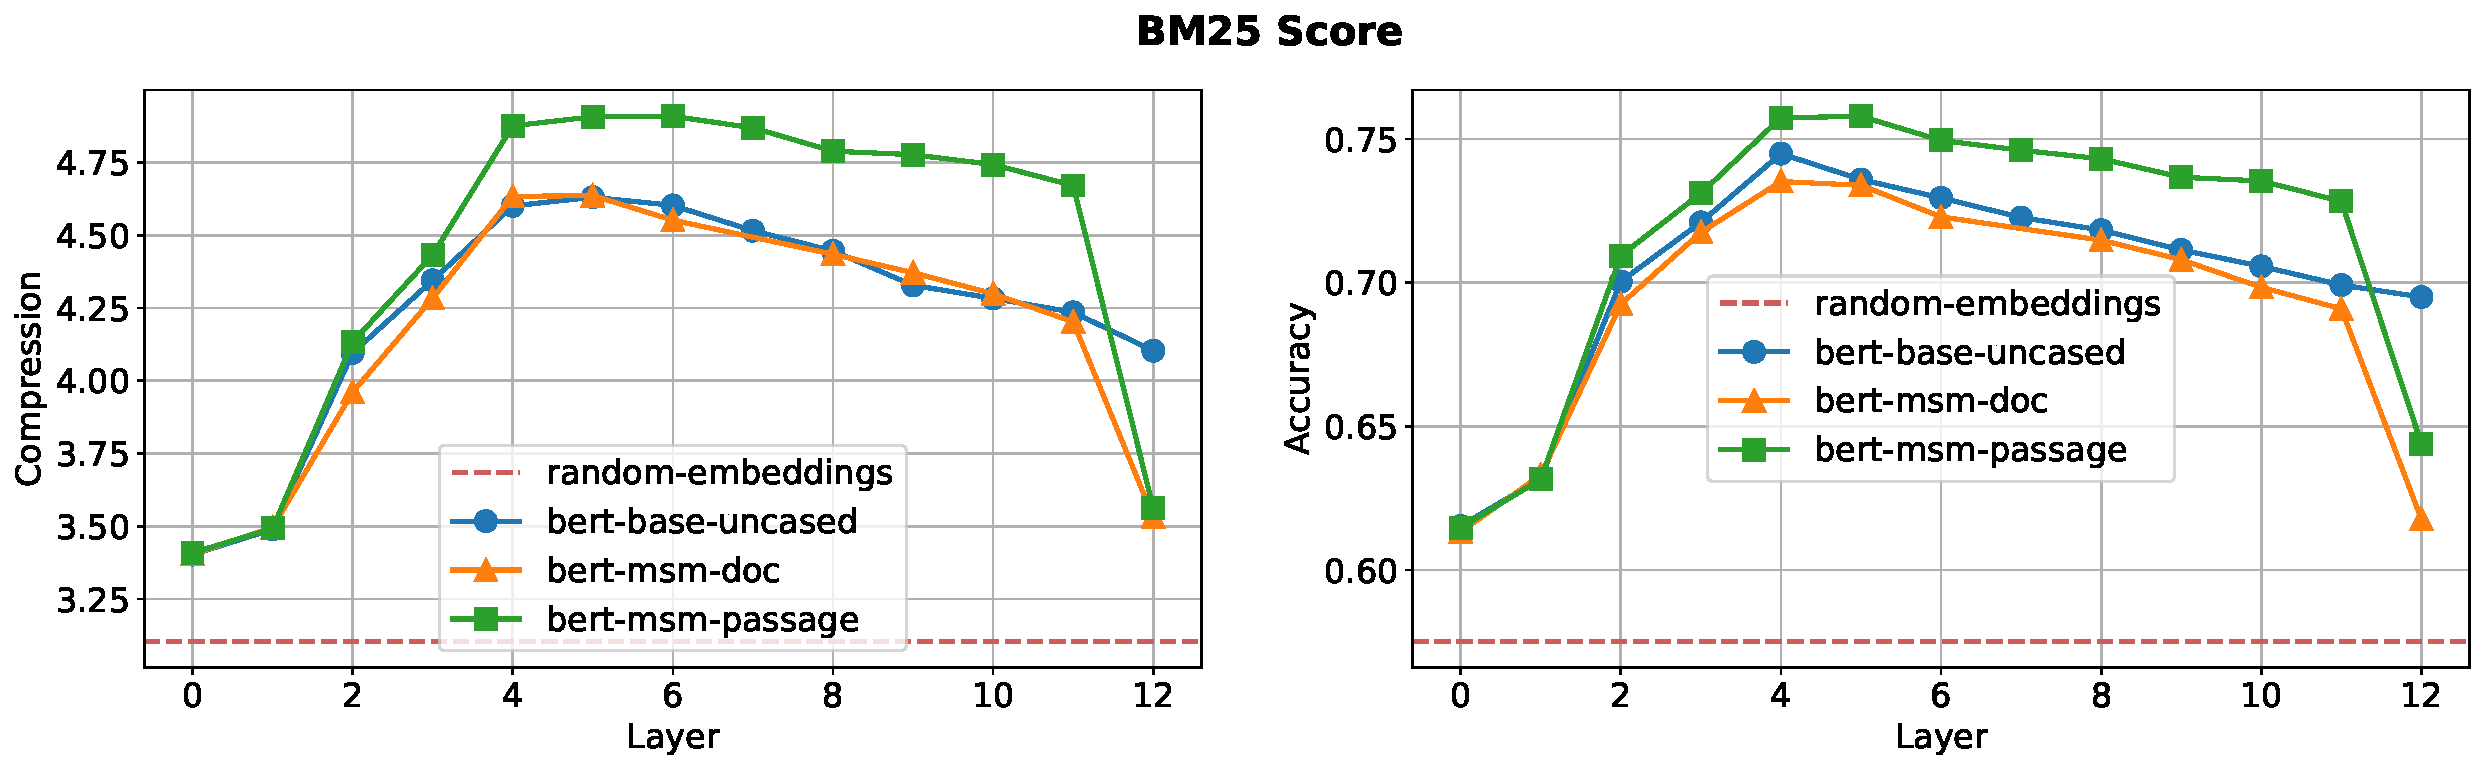
\includegraphics[width=1.25\textwidth]{gfx/probing/bm25}}
    \caption{\dots}
\end{figure}

\begin{figure}
    \label{fig:sem_sim}
    \centering
    \makebox[\textwidth][c]{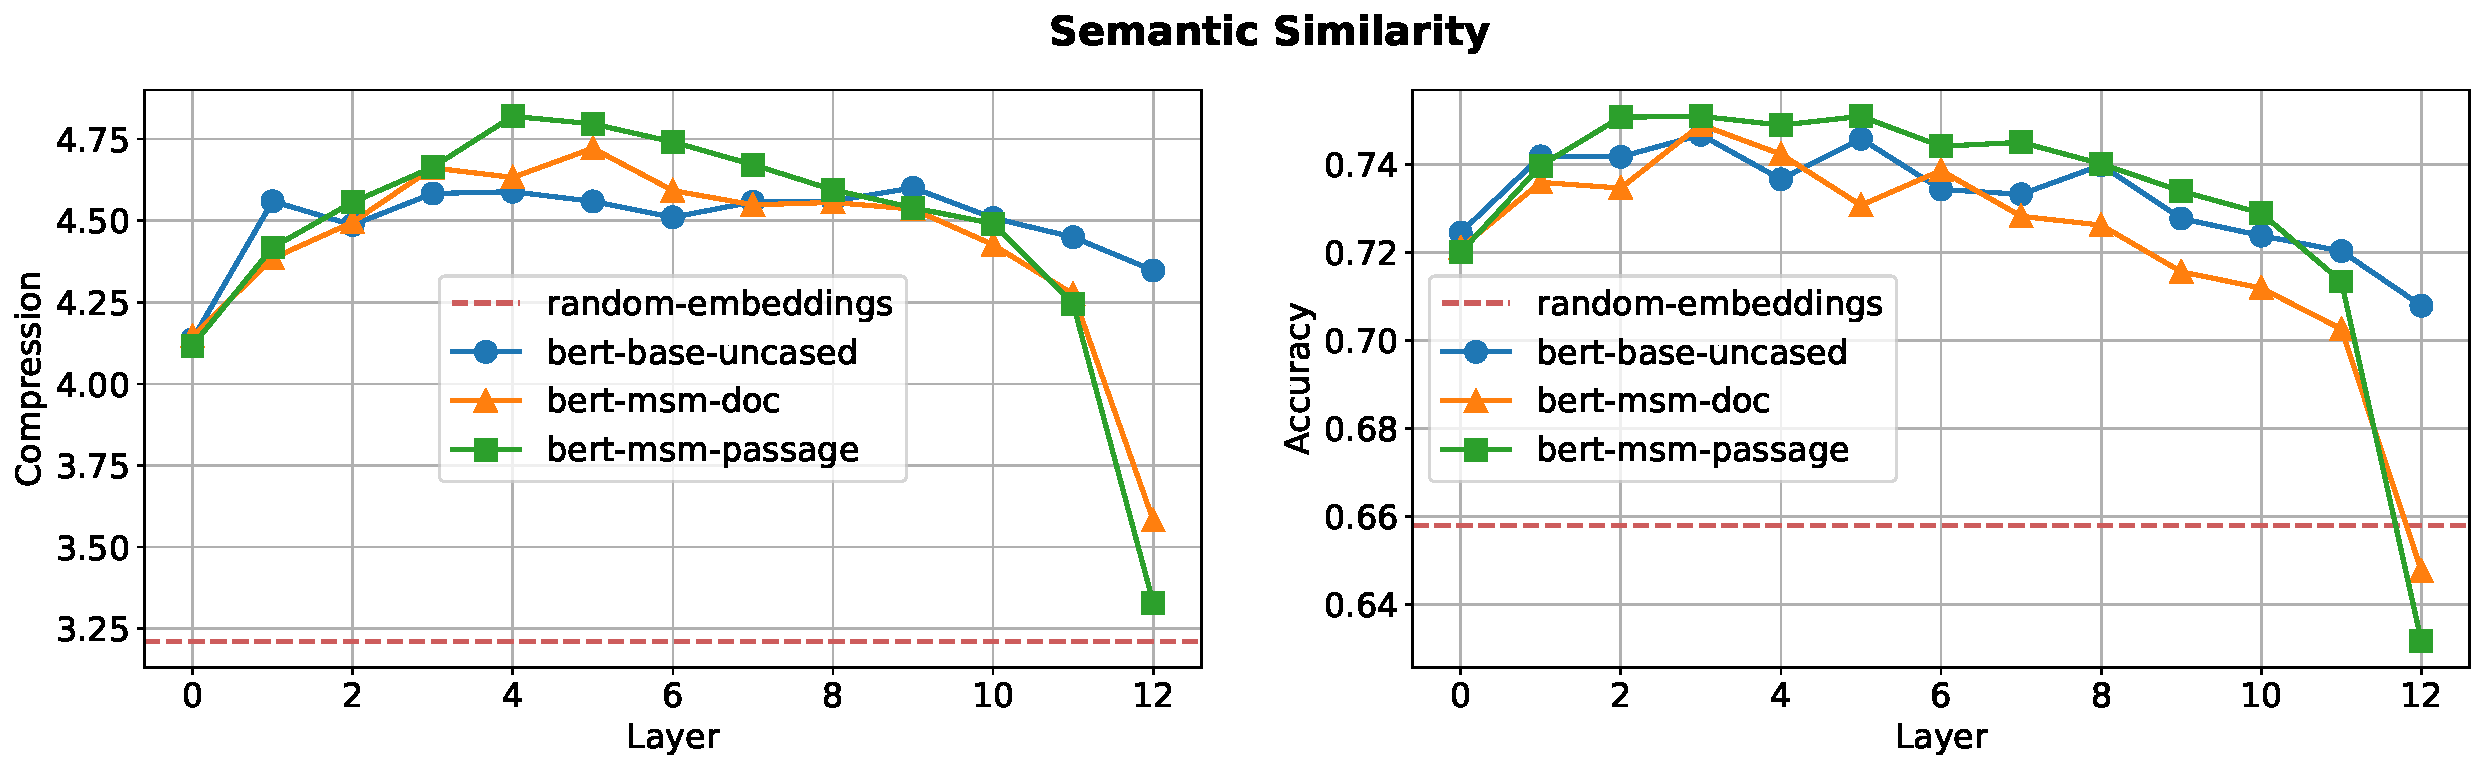
\includegraphics[width=1.25\textwidth]{gfx/probing/sem_sim}}
    \caption{\dots }
\end{figure}

\begin{figure}
    \label{fig:coref}
    \centering
    \makebox[\textwidth][c]{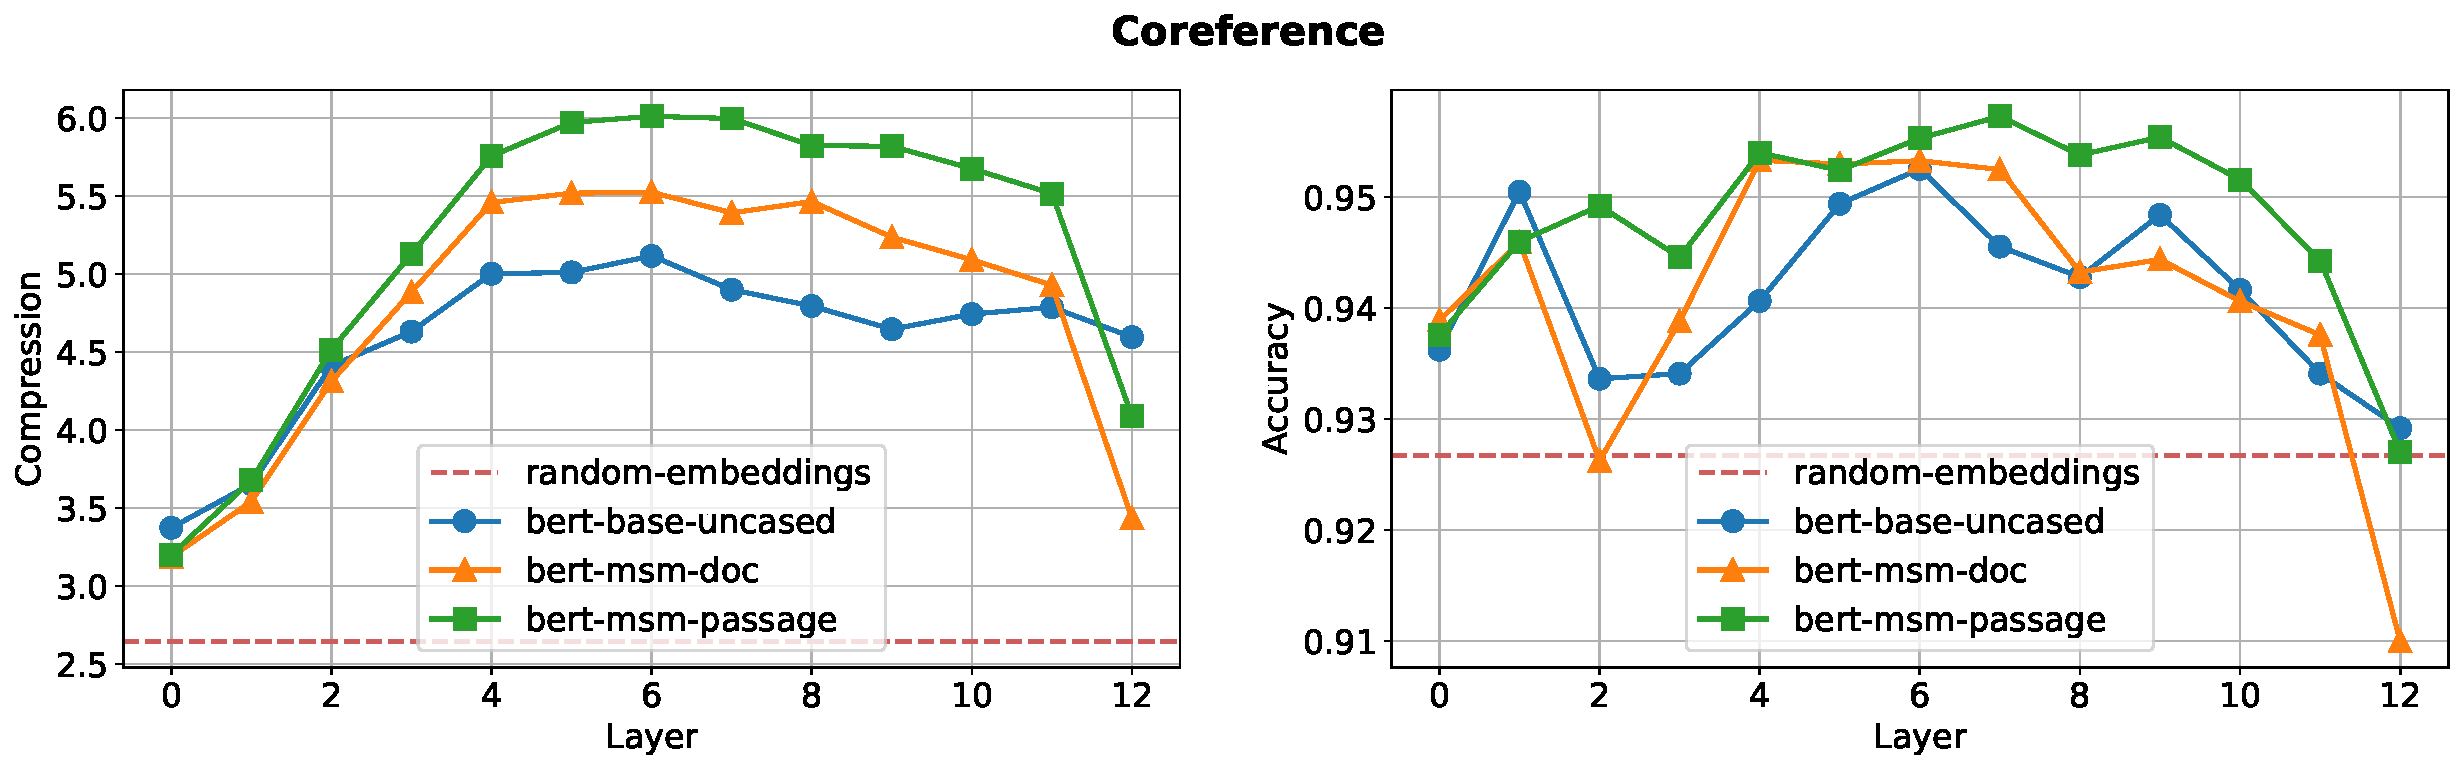
\includegraphics[width=1.25\textwidth]{gfx/probing/coref}}
    \caption{\dots}
\end{figure}

\begin{figure}
    \centering
    \makebox[\textwidth][c]{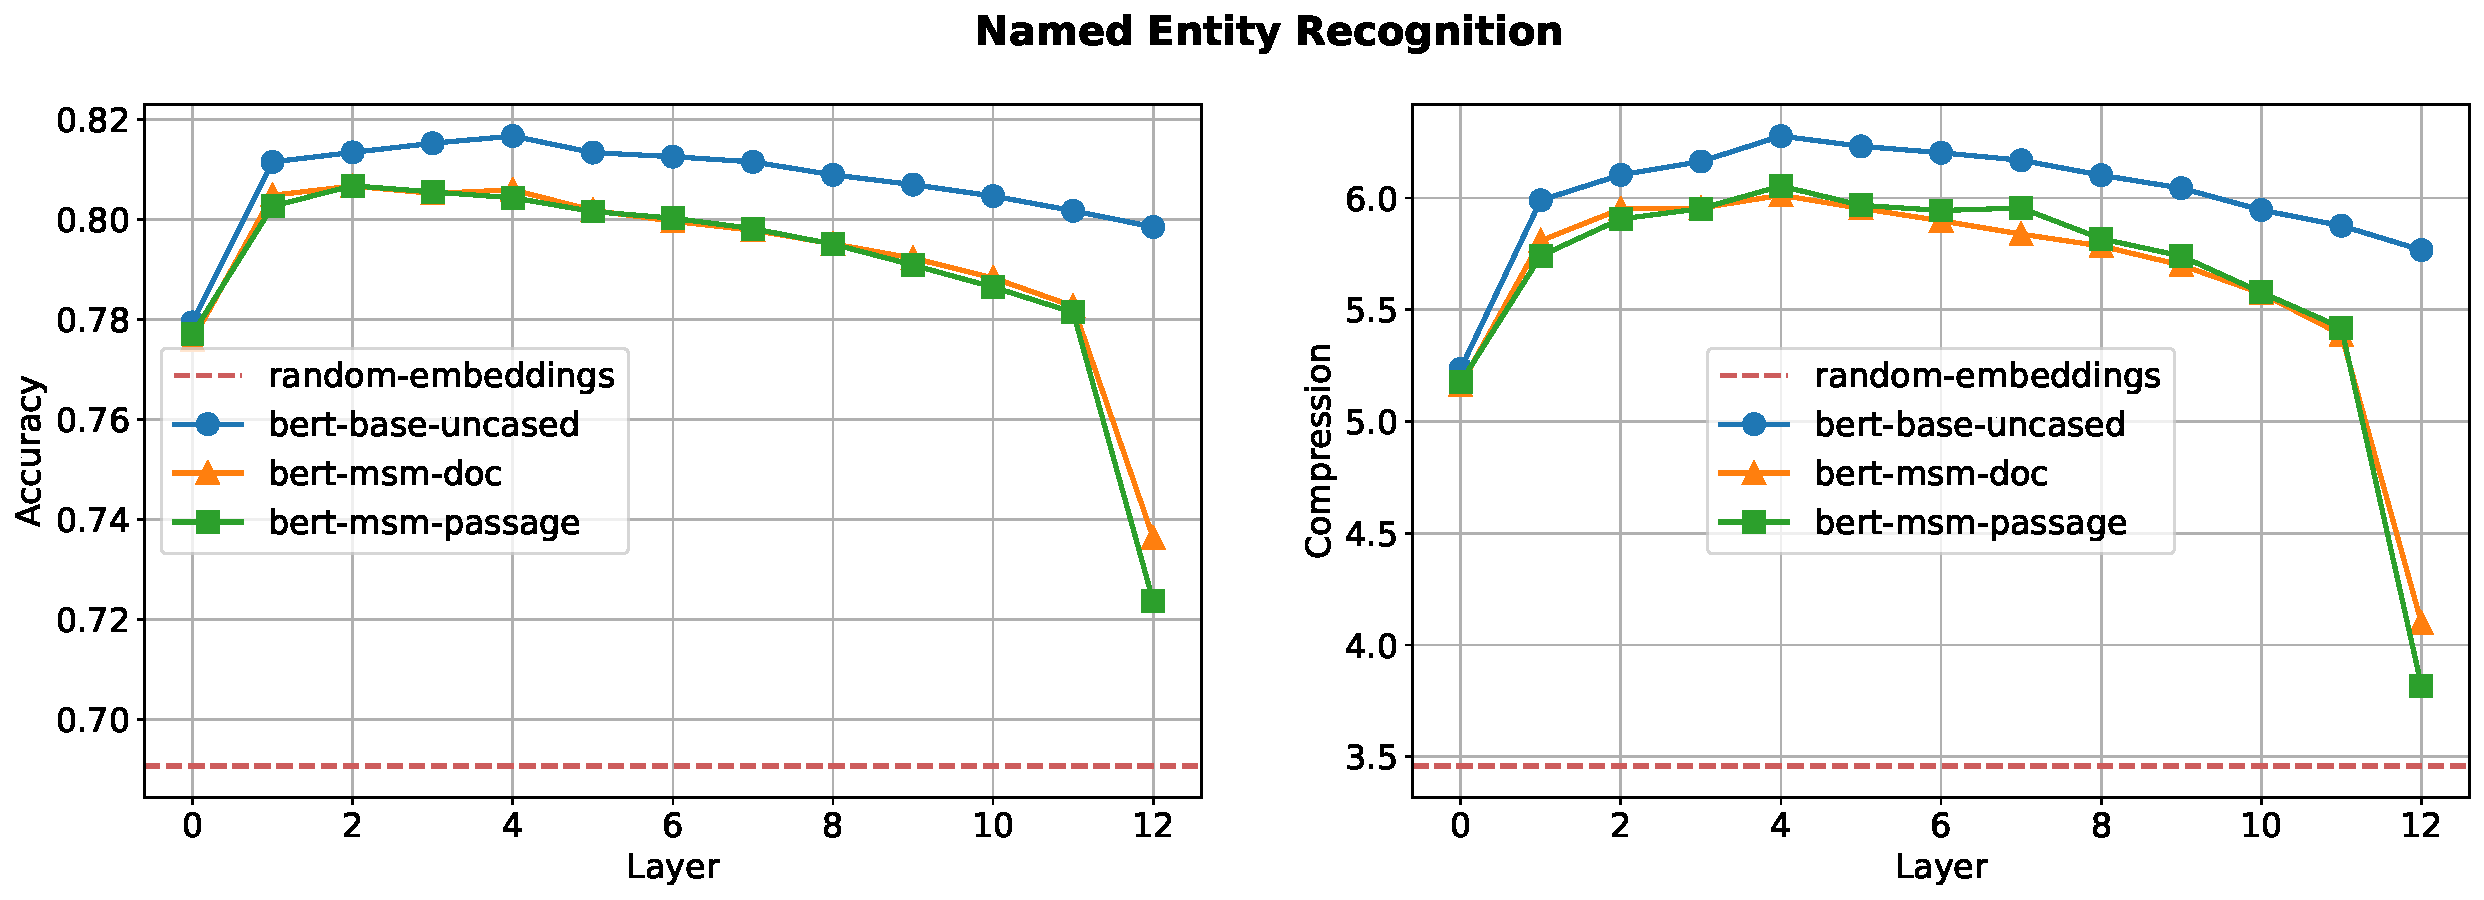
\includegraphics[width=1.25\textwidth]{gfx/probing/ner}}
    \caption{\dots}
\end{figure}

\begin{figure}
    \centering
    \makebox[\textwidth][c]{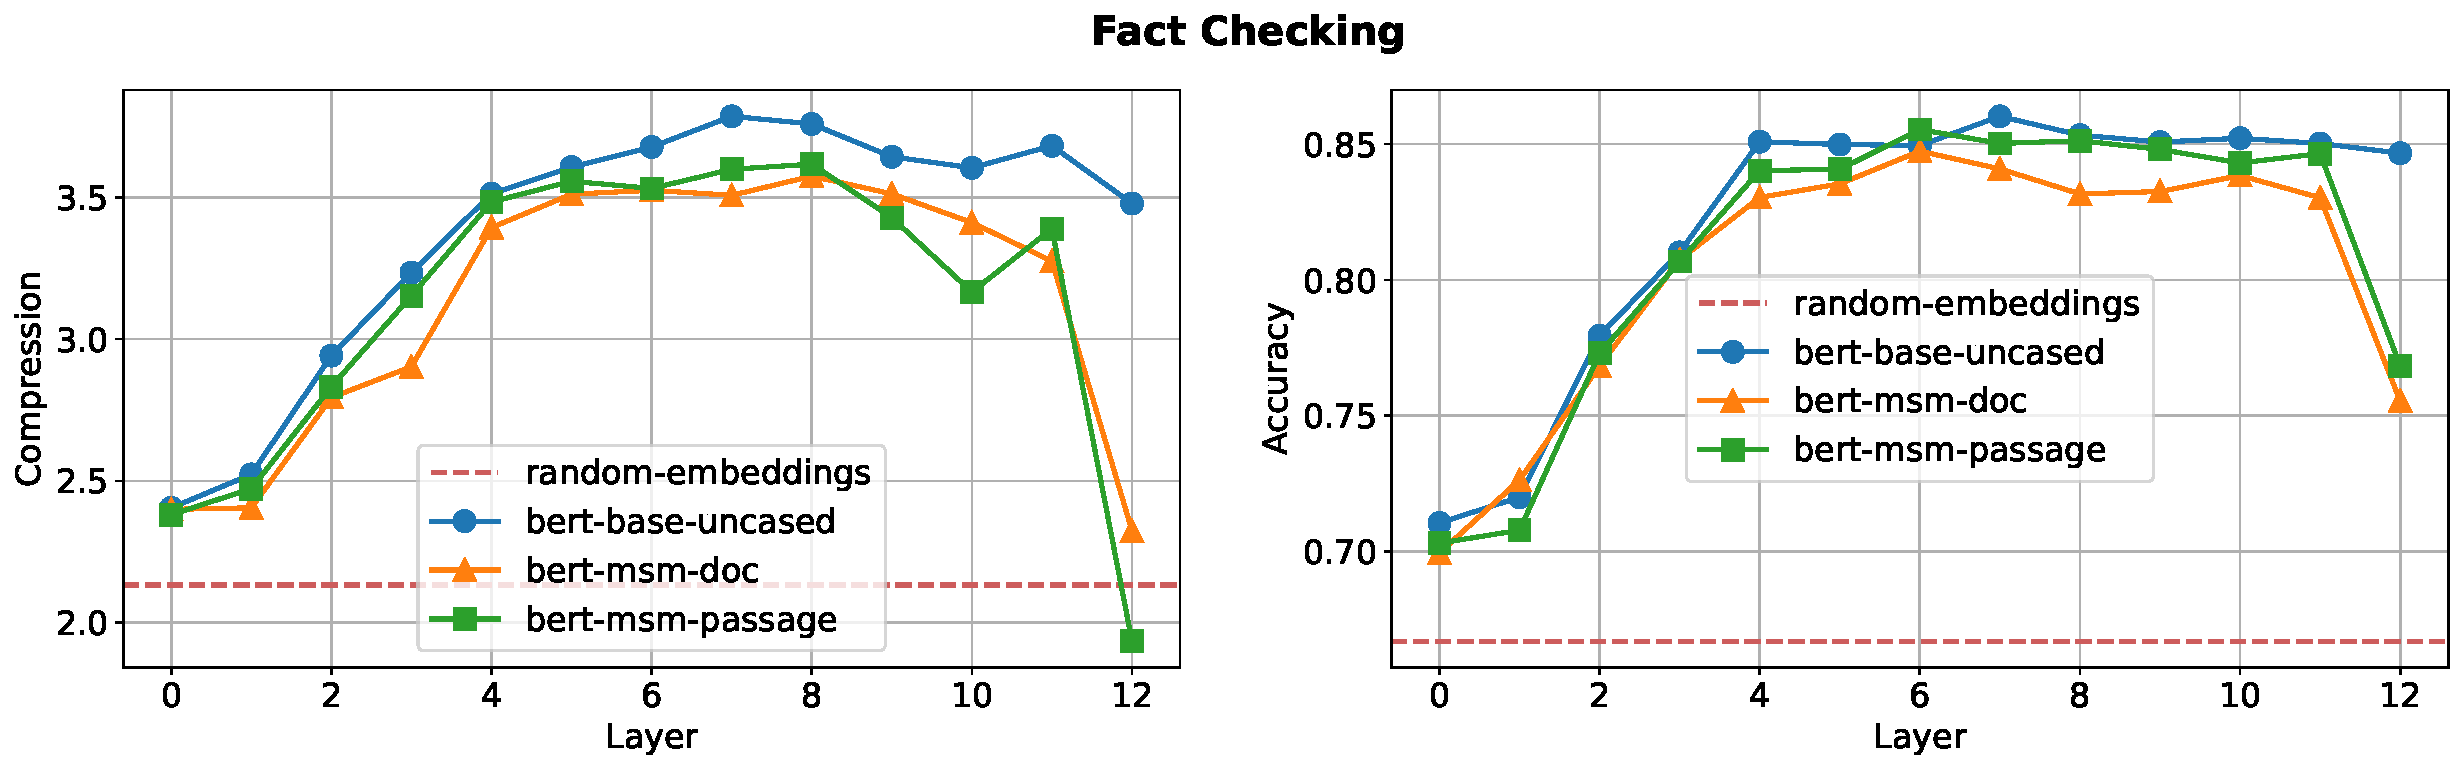
\includegraphics[width=1.25\textwidth]{gfx/probing/fact_check}}
    \caption{\dots}
\end{figure}



\begin{figure}
    \label{fig:heatmap_comp_passage}
    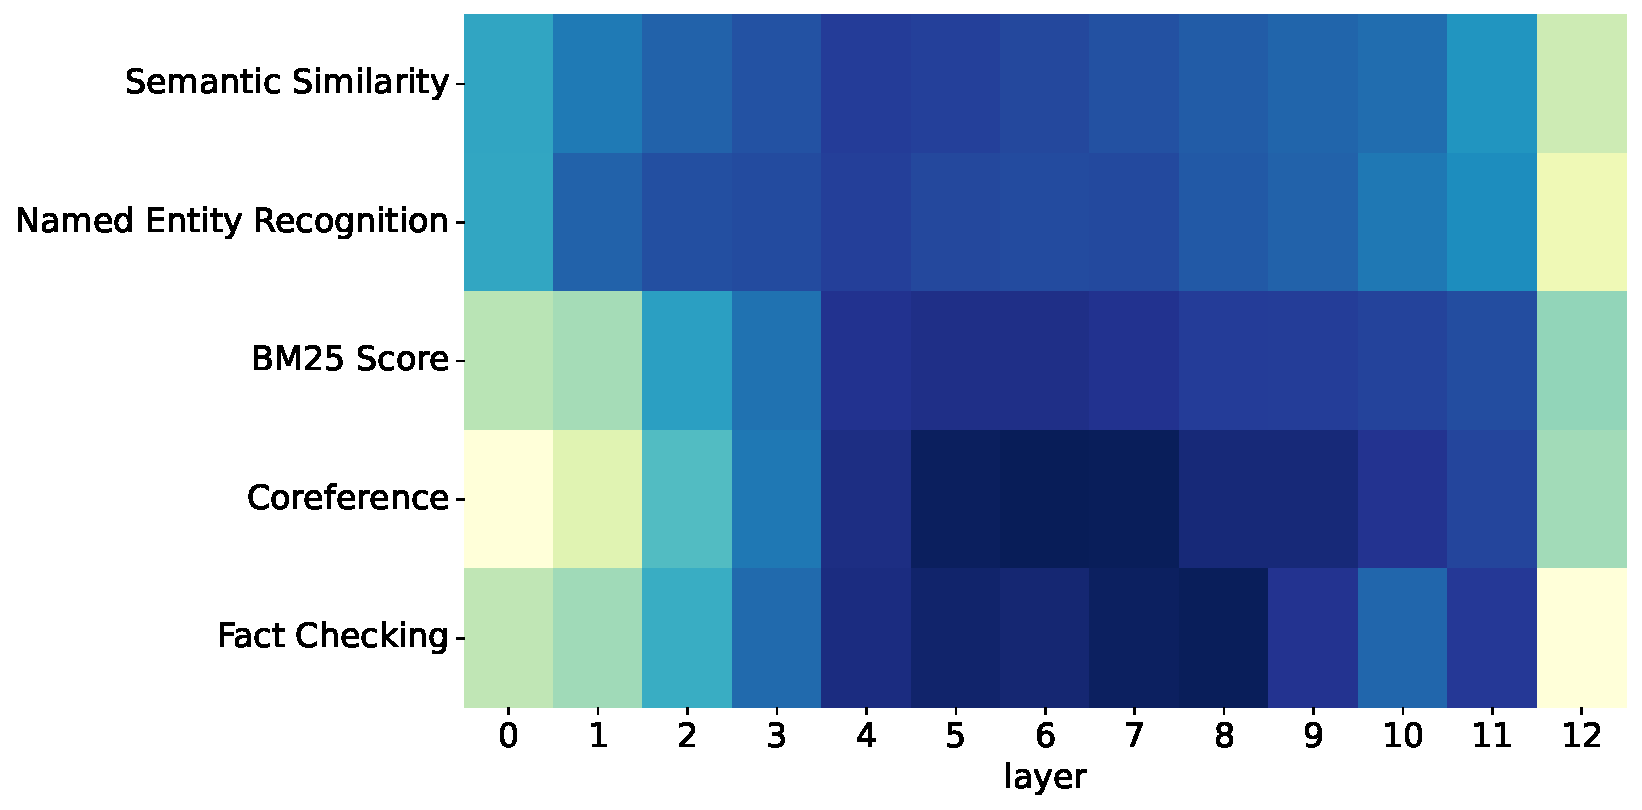
\includegraphics[width=\textwidth]{gfx/probing/heatmap_compression_passage}
    \caption{\ti{bert-msm-passage}: Compression as a function of task and layer, row-normalized. Darker colors represent higher values.}
\end{figure}

\begin{figure}
    \label{fig:heatmap_comp_base}
    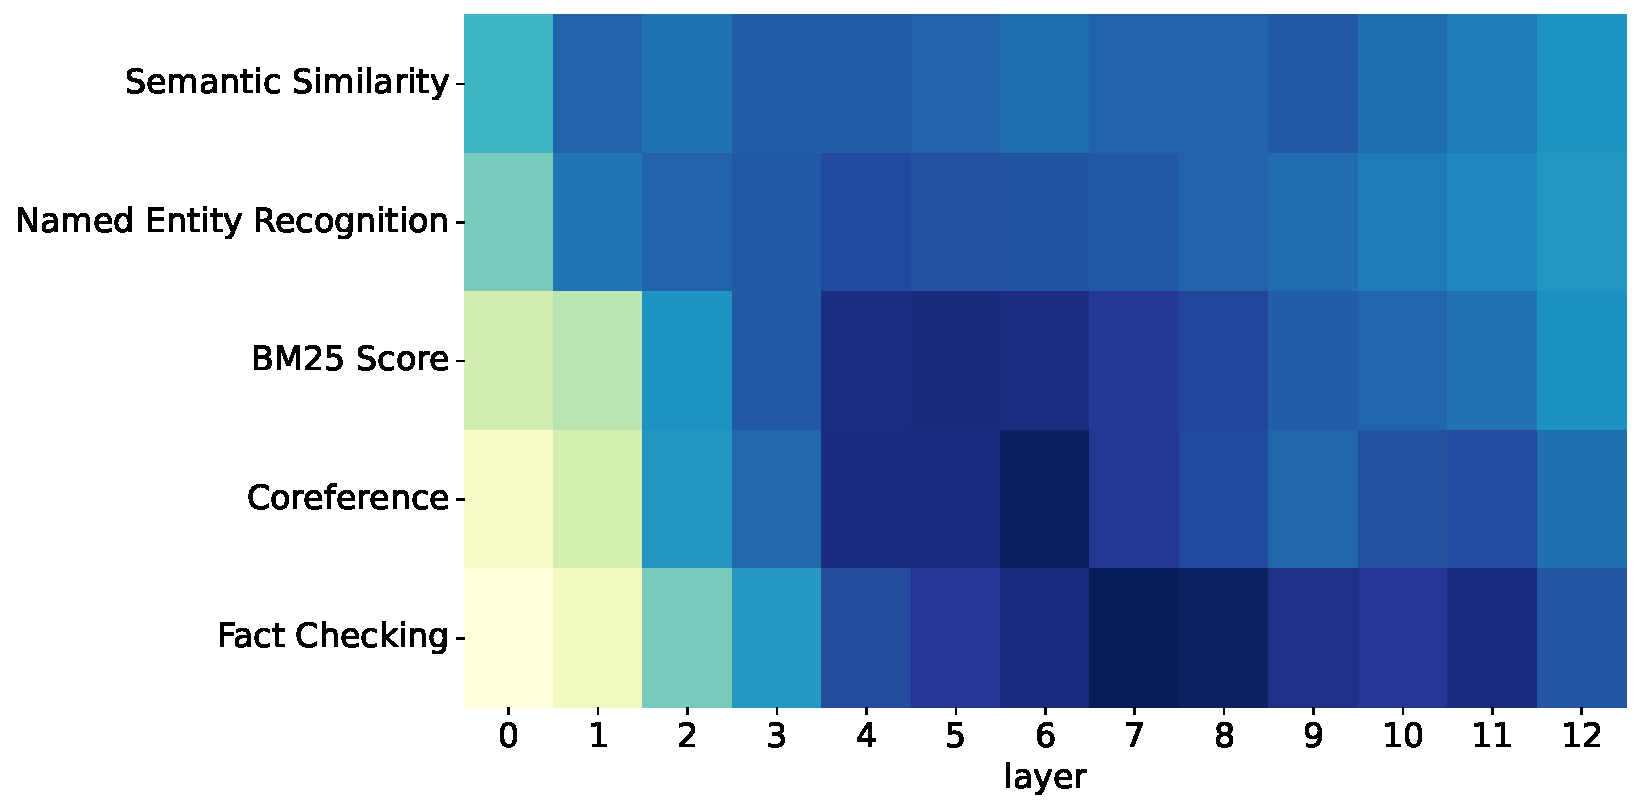
\includegraphics[width=\textwidth]{gfx/probing/heatmap_compression_base}
    \caption{\ti{bert-base-uncased}: Compression as a function of task and layer, row-normalized. Darker colors represent higher values.}
\end{figure}


\begin{figure}
    \centering
    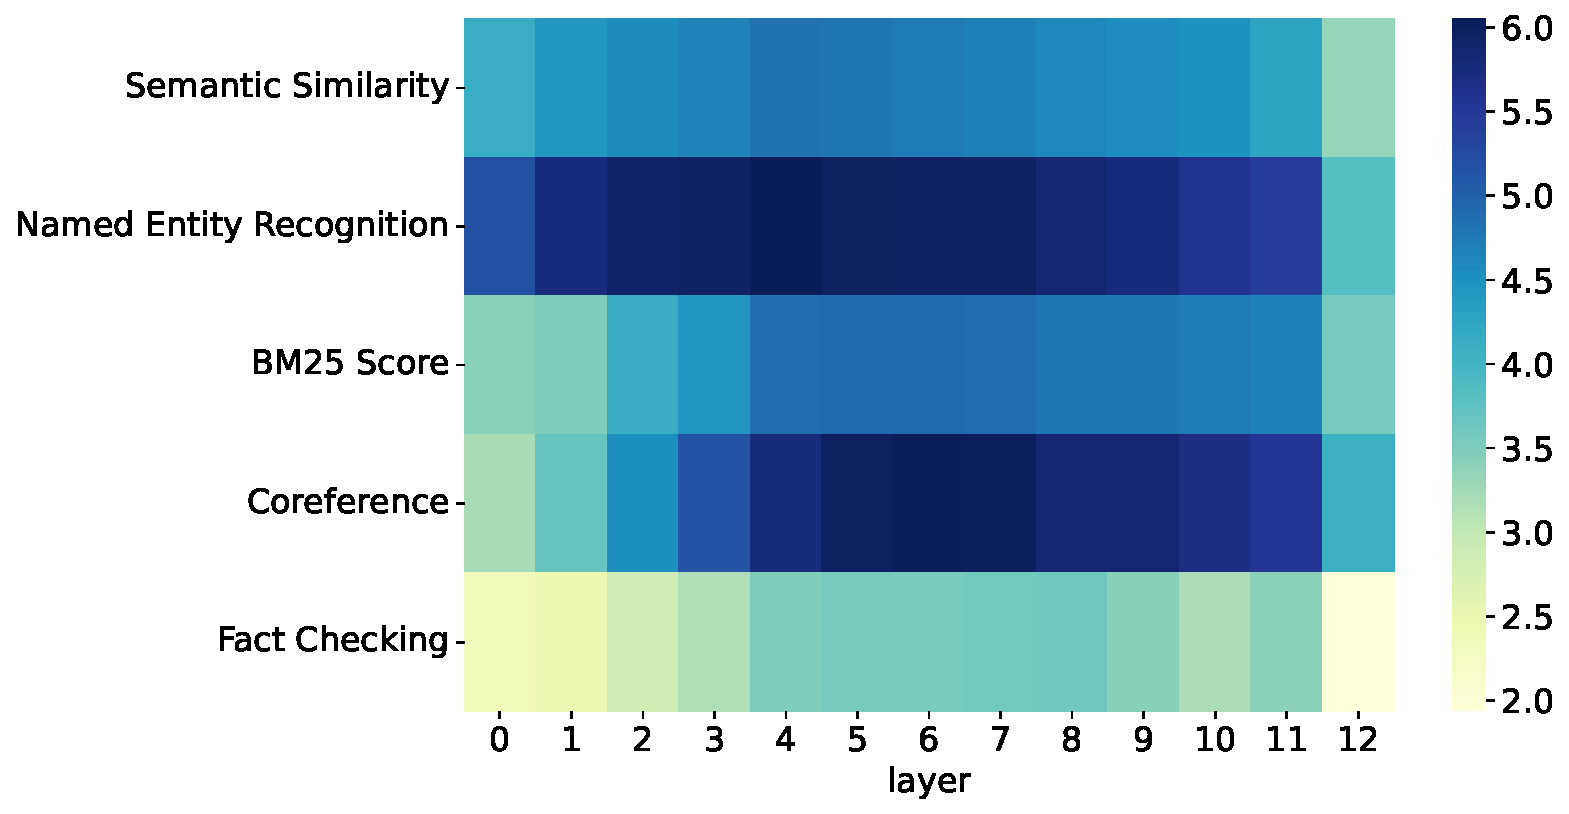
\includegraphics[width=\textwidth]{gfx/probing/abs_heatmap_compression_passage}
    \caption{\ti{bert-msm-passage}: Compression as a function of task and layer, absolute values.}
\end{figure}

\begin{figure}
    \centering
    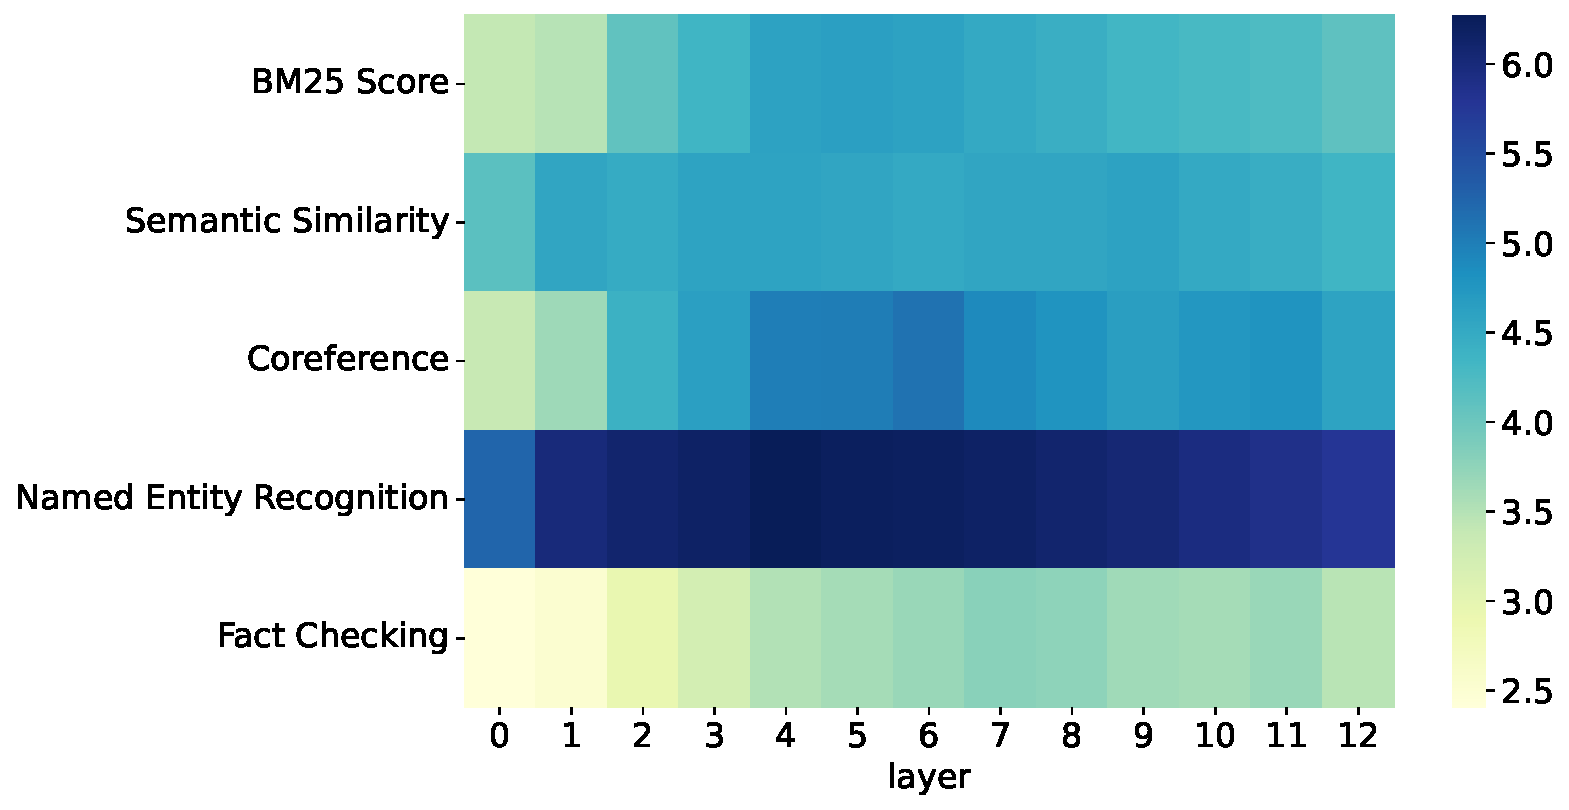
\includegraphics[width=\textwidth]{gfx/probing/abs_heatmap_compression_base}
    \caption{\ti{bert-base-uncased}: Compression as a function of task and layer, absolute values.}
\end{figure}

